\chapter{State-of-the-Art}\label{sec:State-of-the-art}

Digital watermarking is a method that helps protect intellectual property for various types of digital data. 
Since it just marks data but doesn't control access to the data, watermarking is a passive protection tool.
There is a wide range of applications that watermarking can be used for, such as copyright protection, fraud and tamper detection, content management on social networks, etc. 
\textit{Fingerprinting} is used for source tracking. 
It is the special application of watermarking where different recipients of the data get differently watermarked content.
The first watermarking methods were developed for the multimedia domain (images, audio, video) and later extended to other types of digital data such as text, software, relational databases, etc. 

\section{Generic framework for watermarking and fingerprinting}
Digital watermarking consists of two main processes: \textit{insertion (embedding)} and \textit{detection (extraction)}.
The insertion process is in charge of watermark creation and embedding it into the data. 
The output is the marked copy of the data that is publicly distributed. 
Insertion process of fingerprinting embeds the different mark for each distributed copy that is specific for each buyer.
Detection process extracts the watermark from the data. It reports the existence of a watermark in the data given as the input, identifies the owner, or in case of fingerprinting identifies the buyer. 
The data on the input of the detection process can be affected by some benign transformations of the data or malicious transformations made by the attacker. 
The general framework for watermarking (and fingerprinting) is shown in \Cref{fig:framework}.

\begin{figure}
    \label{fig:framework}
    \centering
    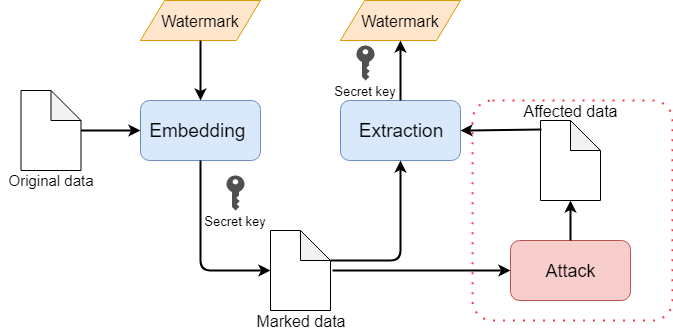
\includegraphics[width=\textwidth]{Figures/framework.png}
    \caption{General framework for watermarking}
\end{figure}

\section{Watermark categorisation}

Digital watermarks may be categorised in several ways depending on different properties. 
The following categorisation criteria are applied to fingerprints as well since we consider fingerprinting as a special case of watermarking. 

\paragraph{Imperceptibility}
The most general categorisation is according to the imperceptibility of a watermark. A digital watermark is called \textit{imperceptible} if the marked copy is perceptually indistinguishable from the original data. 
A watermark is \textit{perceptible} if its presence in the data is noticeable (e.g. owner's logo as an overlay on an image).

\paragraph{Detectability}
Watermark schemes can be categorised in terms of verifiability / detectability, i.e. needing the original data to extract the watermark from the marked data. A \textit{Blind} watermarking scheme does not need the original data for the extraction process, while \textit{non-blind} does. 

\paragraph{Robustness}
Furthermore, according to its robustness, watermarks can be categorised into \textit{fragile}, \textit{semi-fragile} and \textit{robust}.  
Fragile watermarks are commonly used for tamper detection because they fail to be detected after the slightest modification. 
Semi-fragile transformation resists some benign transformations, but fail detection after malignant transformations (attacks). 
Robust watermarks resist a wide range of benign or malignant transformations and satisfy the property that the removal of a watermark is not possible without significantly degenerating the data quality.

\paragraph{Distortion}
In \textit{distortion-based} watermarking techniques marking introduces distortions to the underlying original data. 
On the contrary, \textit{distortion-free} watermarking techniques rely on detecting the watermark as a function of the data itself without changing the original data. 
Distortion-free watermarks are fragile and are applied in tamper detection.

\section{Multimedia, text and software}
The concepts of watermarking \cite{cox1997secure, petitcolas2000information, lee2001survey} and fingerprinting \cite{wu2004collusion} digital data firstly appear in domains of multimedia data and are extensively studied over the last two decades.
Most of these techniques are developed for images \cite{o1996watermarking} and later extended to video \cite{hartung1998watermarking} and audio \cite{boney1996digital,swanson1998robust}.

Image watermarking is applied in two main domains of an image: in the spatial domain where an image is represented by pixels and in the transform domain where it is represented in terms of its frequencies (the image is segmented into multiple frequency bands using a mathematical transform, for instance, Discrete Cosine Transform (DCT), Discrete Wavelet Transform (DWT) and Discrete Fourier Transform (DFT)) \cite{potdar2005survey}.
The watermark can be embedded in the spatial domain by modifying pixel values \cite{nikolaidis1998robust} or adding an overlying layer on top of the original image \cite{piec2014real}, however more robust watermarks are usually embedded in the transform domain by modifying the transform domain
coefficients \cite{suhail2003digital,solachidis2001circularly}.
More advanced watermarking techniques are developed for video watermarking which extends and incorporates watermarking techniques for images \cite{wolfgang1999perceptual,swanson1998multiresolution}. 
Most of the image and video watermarking algorithms focus on processing data files stored on a disc, while some introduce real-time content processing (applied for example on screenshot images) \cite{piec2014real,kang2006implementation}.

There have also been some approaches in applying a watermarking scheme in other domains such as text and software. 
Techniques for watermarking text data typically exploit
special properties of text formatting and semantics. 
Watermarks are often introduced by altering the spacing
between words and lines of text \cite{maxemchuk1994electronic}. 
Other techniques rely on natural language processing and rephrasing sentences in the text \cite{atallah2001natural, atallah2000natural, atallah1999watermarking, atallah2002natural}.
Techniques for watermarking software only have limited success in their native domain \cite{palsberg2000experience,collberg1999software}.
A key problem is that the instructions in a computer program can often be rearranged without altering the semantics of the program. This resequencing can destroy a watermark. 
Techniques have also been proposed to prevent copying of software, but they require installation of tamper-resistant modules in users’ machines, which limits their successful adoption in practice.

\section{Watermarking Relational Databases}
Digital watermarks in the domain of multimedia are not easily extended or adapted to relational database applications, because of the inherent differences between multimedia data and relational databases.
For example, a lot of techniques for images and audio rely on phenomena based on the limitation of the human visual and auditory system. Furthermore, multimedia data contains a large number of redundant bits providing much wider cover for embedding the watermark than it is the case with relational data. 
Relational data may as well consist of multiple types of data - numerical, categorical, text, etc., requiring different approaches for embedding the watermark. 
Categorical data is known to introduce additional issues for watermarking compared to numerical, so we will divide these techniques into separate subsections.
Therefore, techniques for watermarking relational data differ significantly from those for multimedia. 
A couple of surveys \cite{rathva2013watermarking,mehta2014watermarking,iftikhar2015survey,kamran2018comprehensive} list most of the proposed watermarking techniques in the literature and classify them, comparing thereat their main properties and robustness to attacks. 
In the remainder of the section, we present the watermarking techniques for relational data, according to the categorisation illustrated in \Cref{fig:categorization} \cite{halder2010watermarking}. 
The first level of categorisation is a distinction of watermarks based on distortion. Distortion-based watermarks are then divided into categories based on the type of data they apply to. A further distinction is made among the techniques applied to a numerical type of data according to what carries the watermark information. 

\begin{figure}
    \centering
    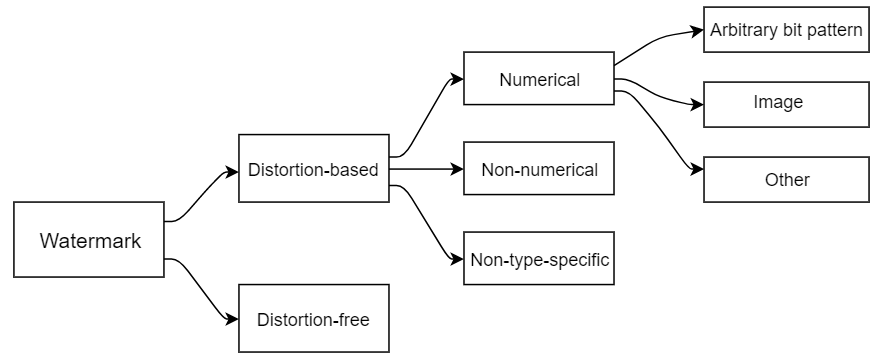
\includegraphics[width=\textwidth]{Figures/categorization.PNG}
    \caption{Categorization of watermarking techniques for relational data}
    \label{fig:categorization}
\end{figure}

\subsection{Distortion-based watermarks}
\subsubsection{Watermarking numerical data}
\begin{enumerate}[leftmargin=*]
    \item \textit{Arbitrary bit pattern as watermark information}
\paragraph{}
Pioneering work on watermarking relational databases is proposed by Agrawal and Kiernan \cite{agrawal2002watermarking}. It is a blind, bit-resetting technique where the watermark insertion is controlled by a gap parameter $\gamma$ (the ratio of tuples to be fingerprinted). 
They use a message authentication code (MAC) - a one-way hash function that depends on a secret key to determine which tuples will be marked. 
The same value $\mathcal{F}(r.P)=\mathcal{H}(\mathcal{K}||\mathcal{H}(\mathcal{K}||r.P))$ is used for selecting the tuple, attribute and bit that will be marked, where $\mathcal{H}$ is a hash-function, $\mathcal{K}$ is a secret key, $r.P$ the primary key of the tuple and $||$ is representing a concatenation.
The important property of a hash function is that it is easy to calculate a hash value (output) for a given input, but computationally difficult to do the reverse. 
Therefore only the owner knowing the secret key can detect where the marks are embedded in the data.
\paragraph{}
This work is extended in \cite{agrawal2003system, agrawal2003watermarking} by introducing a pseudo-random sequence generator instead of the MAC in the process to select tuples, attributes and bits for watermarking.
The technique from \cite{agrawal2003watermarking} (referred to as the AKH technique; AKH stands for the initials of the authors) and its predecessor \cite{agrawal2002watermarking} is used for many extended works in watermarking and fingerprinting relational databases.
The technique in principle contains two steps: watermark insertion and watermark detection, according to the generic framework for watermarking. 

The \textit{watermark insertion algorithm} marks certain numerical attributes such that the least significant bits (LSBs) are altered, therefore this technique assumes that the dataset contains one or more numerical attributes.
The database owner is left to decide the number of LSBs available for marking $\xi$, such that the changes of marked attributes stay imperceptible. 
The insertion algorithm then uses a cryptographic pseudo-random sequence generator $\mathcal{G}$, seeded by a secret key known only to the owner of the database, and concatenated with the primary key attribute value of each tuple from a database. 
The main assumption that the AKH technique relies on is the existence of a primary key in the dataset. 
Li et. al. \cite{li2003constructing} propose three different schemes to obtain a virtual primary key for relational databases without primary key.
The numbers generated by $\mathcal{G}$ determine the tuples, attributes within the tuples and LSBs within the attribute values to be marked, as well as the mark itself. 
It is computationally infeasible to predict the next number in the cryptographic pseudo-random sequence.
Thus, it is computationally infeasible to guess the marking pattern without the knowledge of the owner’s private key. 

The \textit{detection algorithm} contains calculating the sequence using a cryptographic pseudo-random sequence generator with the same seeds as in the insertion algorithm. 
Those sequences will be the same because repeated executions of the generator seeded by the same value always produce the same sequence. 
Thus, the detection algorithm finds which bits within the database should have been marked and counts how many of them match the bits from the database suspected for piracy. 
If the number of matches is “large”, the database owner can suspect the piracy. 
On the other hand, if the matching is “too small”, the database owner can suspect that the attacker somehow identified the marking pattern and recreated the original database values.
The number of matches necessary for suspecting piracy is defined by a parameter $\tau$ called \textit{significance level}. 

The authors analysed the robustness of this technique against several malicious attacks, namely, subset attacks, bit-flipping attacks, mix-and-match attack and false claim of ownership. 
More of the robustness analysis of the AKH scheme is done in later work by Lafaye \cite{lafaye2007analysis}.
\paragraph{}
Extensions and improvements to the AKH technique have been proposed in \cite{qin2006watermark} and \cite{gupta2009database}. 
The first one \cite{qin2006watermark} improves the AKH by using chaotic random series based on the Logistic chaos equation instead of a hash function. 
This has two advantages: non-repetitive iterative operation and sensitiveness to initial values in a way that the selection of bits meets the requirements of both data range and data precision of each attribute, rather than using same $\xi$ for all attributes as it is the case in the AKH. 
This strategy's advantages manifest by a significantly decreased error when data with large differences in ranges within the attributes is watermarked. 
Another extension is a reversible version of the AKH watermarking scheme \cite{gupta2009database} where watermark can be recovered during the detection phase and the attribute can be restored to its unmarked value.

The watermarking method in \cite{xiao2007second} embeds random digits at second LSB positions of the numeric candidate attributes. The watermark is not explicitly embedded like in the previously mentioned techniques, but rather used for identifying valued groups of tuples to embed the random values.

\item \textit{Image as watermark information}

There is a couple of proposed techniques that mark the data using an image as watermark information.
\paragraph{}
The method in \cite{wang2008atbam} describes embedding the scrambled image based on the Arnold transform with scrambling number \textit{d}. 
The scrambling number improves the security of this technique because of it an additional parameter, besides the secret key, that the embedding scheme relies on.
The scrambled image is represented as a binary string and embedded into tuples that are previously grouped using hash values depending on a secret key, primary key and the order of the image. 

Another method \cite{hu2009image} follows the similar algorithmic steps as in \cite{wang2008atbam}, but embeds the original image converted into a bit flow instead of a scrambled image.

The method in \cite{zhou2007additive} divides an image into \textit{header} and \textit{image data}  in the insertion phase. The header is used in a hash function together with tuple's primary key to determine tuple's ID value and determine positions where the image data will be embedded.

\item \textit{Other types of watermark information}

Besides arbitrary meaningless bit pattern and image as watermark information, other types of watermark information have been proposed and embedded into the data.
One example is speech as a watermark information \cite{wang2008speech}. The proposed technique uses compressed owner's speech converted into a bitstream as a watermark and follows similar algorithmic steps as \cite{hu2009image}.
Furthermore, in \cite{cui2008approach} authors propose a Genetic Algorithm-based technique to generate watermark signal, in \cite{zhang2005method} the cloud watermarking scheme is proposed and authors in \cite{huang2009cluster} use \textit{k-means} algorithm to cluster the tuples into some equivalent classes.

Watermark information may as well be the content of data itself \cite{zhang2006relational, guo2006fragile}.
Generally, some bits of one part of the data, i.e. characteristics are extracted in the insertion phase and used to mark the other parts of the data. 
\end{enumerate}

\subsubsection{Watermarking non-numerical data}
Non-numerical data requires different techniques for watermarking purposes than numerical data because of its discrete nature. 
The concept of introduced errors is perceived differently as well because we cannot apply the same measurements as in the case of categorical data, e.g. marking the numerical value 23 as 25 does not have the same impact on the data as marking "blue" as "red". 
The latter may not even be acceptable in some settings, therefore watermarking non-numerical data needs to start from the assumption that the user accepts this kind of errors and that they do not violate credibility and utility of the data. 
Another limitation of watermarking categorical data that can cause the loss of credibility is the semantic correlation between the attributes that depending on the setting needs to be preserved.

In \cite{sion2004proving,sion2005rights} the authors propose a technique for watermarking categorical data.
The technique requires the presence of a primary key in the dataset.
The embedding process relies on two secret keys $k_1$ and $k_2$.
The first secret key $k_1$ is used for selecting the tuples "fit" for watermarking together with parameter $e$ and the primary key. 
$e$ is a control parameter of how many tuples get marked, i.e. has the same purpose as parameter $\gamma$ in schemes for watermarking numerical data. 
The number of tuples "fit" to be marked ($\eta/e$) is usually larger than the size of a watermark, which is solved by converting the watermark $wm$ into $wm\_data$ of length $\eta/e$ using an Error Correcting Code (ECC). 
In every "fit" tuple, the embedding algorithm generates a secret value in bit representation. 
The number of bits in a secret value is equal to the number of bits required to represent all possible categorical values for the attribute. 
The least significant bit of the value is marked by a randomly chosen bit of $wm\_data$ depending on the primary key and the secret key $k_2$. 
The marking scheme assures that the resulting categorical value will be some value from the domain of the attribute.
The pseudo-random nature of the choice of a bit from $wm\_data$ guaranties that almost all bits will be chosen at least once during the embedding process. 
Using two different secret keys $k_1$ and $k_2$ assures non-correlation between the selected tuples for embedding and the corresponding bit value positions in $wm\_data$. 

The detection algorithm reverses the operations from the insertion phase and extracts some $wm\_{data}'$. Once $wm\_{data}'$ is available, the ECC is invoked to generate the "closest" or "most likely" corresponding watermark $wm$. 

The authors also suggest an embedding scheme based on multiple categorical attributes by considering not only the association between the primary key and a single categorical attribute but also associations between different categorical attributes. 
The embedding scheme described previously is applied for every combination of \textit{primary key - categorical attribute}, and every combination of two categorical attributes. In combinations of two categorical attributes, one of them serves as a virtual primary key for the embedding process. 
For instance, let us have a dataset containing primary key \textit{K} and two categorical attributes $C_1$ and $C_2$. 
The embedding scheme will be performed 3 times, for $(K,C_1)$, $(K,C_2)$ and $(C_1,C_2)$. 
First, two runs of the embedding scheme will use the secret key $k_1$, $e$ and the primary key $K$ for the choice of tuples to be marked and embeds the mark in attribute $C_1$ (or $C_2$ for the second combination).
The embedding scheme run for $(C_1,C_2)$ uses the secret key $k_1$, $e$ and attribute $C_1$ for the choice of tuples to be marked and embed the mark in attribute $C_2$.
In this scheme for watermarking multiple categorical attributes, taking just described case, we can see that markings for $(K,C_2)$ interfere with markings for $(C_1,C_2)$. 
Even though this scheme is claimed to be robust against serious attacks (e.g. vertical data partitions) and breaks the dependency of the primary key, the convenience of this method is questionable due to the increase of the number of combinations (sequence of triangular numbers) for more categorical attributes in the dataset.

This watermarking technique is applied to binned medical data in \cite{bertino2005privacy}.

Another method for watermarking non-numerical data has been proposed in \cite{al2008robust}, for non-numeric multi-word attributes. The watermarking scheme is based on hiding a binary image in space of non-numeric multi-word attributes of subsets of tuples by introducing double spaces on pseudo-randomly chosen places. The scheme is claimed to be robust against subset and superset attacks, however, it may suffer from the simple malicious action that replaces all double spaces between two words by a single space and therefore erases the watermark.  

\subsubsection{Watermarking non-type-specific data}
Techniques have been proposed to use fake tuples \cite{pournaghshband2008new} or fake attributes \cite{prasannakumari2009robust} as watermark information. 

The approach from \cite{pournaghshband2008new} generates fake tuples and inserts them erroneously into the dataset. 
The fake tuple creation algorithm uses Bernoulli sampling probability to decide whether the new value will be chosen from the existing set of values of the corresponding attribute, or a set of fake values. 
The choice of the new value can be made uniformly, or as the value with higher-occurrence frequency in the existing set of values of the corresponding attribute in the relation. 
The detection algorithm checks via the primary key to see whether the fake tuples inserted during watermarking insertion phase exist or has been changed. As soon as it finds one match, detection is done. 
The detection fails for the watermarked database when all of the fake tuples are deleted.
One advantage of this scheme is that the owner can be publicly verified more than once until all of the fake tuples are revealed.
Another advantage is that this scheme works with all types of values - numerical, categorical, dates, etc.

The technique of inserting a virtual attribute in the relation which serves as watermark \cite{prasannakumari2009robust} generates new values as aggregates obtained from any other numerical value from the dataset. 
This approach is fragile and can easily detect any of the deletion, insertion or alteration attacks, however, it suffers from the watermark removal attack.  

\subsection{Distortion-free Watermarking}
The watermark information may be the hash value extracted from the data.      
The main idea is to partition the data in some way. 
\cite{li2004tamper} propose a technique where partitioning of tuples is based on the hash value parameterized with the primary key and secret key, whereas in \cite{bhattacharya2010distortion}, partitioning is based on categorical attribute values. 
After partitioning, hash values for each group as well as tuple level hash values are computed. Based on the hash values and their parity, two tuples' order changes or doesn't. 
These schemes are able to detect any modifications made to a database relation.

There are other proposed solutions in the literature that are used as watermark information, such as combining owner's mark and database features \cite{tsai2006database}, converting database relation into binary form \cite{li2006publicly,bhattacharya2009generic} or R-tree based permutations \cite{kamel2009schema}.

Most of the distortion-free watermarking techniques are fragile, i.e. they aim at maintaining the integrity of the information in the database in addition to the ownership protection. 
The watermark insertion phase does not depend on any specific type of data and does not introduce any distortion in the underlying data of the database.

\section{Fingerprinting Relational Databases}

Fingerprinting is a special application of watermarking - a distinct watermark (a fingerprint) is generated and embedded in every distributed copy of the data. 
In paper \cite{kamran2018comprehensive}, the authors gave a classification and brief analysis of relevant watermarking and fingerprinting techniques. \Cref{tab:comparison_fingerprinting} is derived from this survey. 
In our review we mention many of the techniques from \cite{kamran2018comprehensive} and include some that are not mentioned in the survey.

Li et al. in \cite{li2005fingerprinting} extended the watermarking technique proposed by Agrawal et al. \cite{agrawal2003watermarking} into a fingerprinting technique.
The marking scheme embeds different bit-strings - \textit{fingerprints} in different releases of data.
The owner generates buyer’s fingerprint from the owner’s secret key and the buyer’s serial number using a cryptographic hash function.
This method of generating the fingerprints avoids storing buyer-fingerprint pairs and additional security management for this database.
Similarly to the watermarking technique \cite{agrawal2003watermarking}, this fingerprinting technique consists of the insertion algorithm and detection algorithm. 

The insertion algorithm follows the steps for selecting the tuple, attribute, LSBs and marks in the same manner as the insertion scheme from \cite{agrawal2003watermarking}, and additionally embeds the generated fingerprint by XOR function applied on the mark (in this algorithm called \textit{mask}) and a selected fingerprint bit. 

The aim of the detection algorithm of the fingerprinting methods, in general, is to determine whether the suspicious database is pirated, as well as to identify the source of the unauthorised release of the database. 
The detection algorithm from \cite{li2005fingerprinting} reverts the fingerprint insertion process similarly to \cite{agrawal2003watermarking}. It locates the bits that should have been altered and compares the matching of the extracted fingerprint with buyers’ fingerprints. 
The exact bit matching of the extracted fingerprint to some buyer’s fingerprint implies this buyer to be an unauthorised distributor.
$\tau$ is a parameter related to the assurance of the detection process.
\paragraph{}
In \cite{liu2004block}, authors propose a block-oriented fingerprinting scheme for relational databases inspired by a fingerprinting scheme for images from \cite{das2002robust}. 
This method also relies on altering the LSBs at certain locations in the database. 

In the insertion algorithm, the LSBs of numerical values from the database (as much LSBs as it is allowed to change) are combined into a two-dimension image and separated into blocks of size $\beta\times\beta$. 
Then a pseudo-random number generator is used to decide the block and position within the block where the fingerprint should be embedded until all blocks are marked. 
Fingerprint bits will be embedded again if there is still unmarked blocks left when all fingerprint bits have been embedded. 
A fingerprint is produced in the same manner as in previous techniques, using the cryptographic hash function seeded by the owner’s secret key and the user’s serial number.

Detection phase consists of sorting the suspicious database according to the primary keys and filling out the database with the original values in case of deletion. 
The location where the fingerprint bit is supposed to be is calculated as in insertion algorithm and the bit is recorded. 
As the fingerprint is embedded multiple times in the dataset, if most of the detected values for a single fingerprint bit are 1, the detected fingerprint is said to be 1, otherwise 0. 
\paragraph{}
Authors of watermarking and fingerprinting system \textit{Watermill} \cite{constantin2005watermill, lafaye2008watermill} further extend the methods from \cite{agrawal2003watermarking} and \cite{li2005fingerprinting} by considering the constraints of data alteration and treating fingerprinting as an optimisation problem. 
By using a declarative language, the usability constraints that the fingerprinted dataset must meet are specified. For example, a purchaser may require that joins between some attributes should be preserved, or that values of some attribute cannot be altered more than a predefined amount. 
One of two proposed fingerprinting strategies consists of translating the weight-independent constraints into an integer linear program (ILP) and using the ILP solver to solve it. 
The second fingerprinting strategy is \textit{pairing heuristics} for larger datasets where using ILP solver might not be efficient.

\paragraph{}
In \cite{guo2006fingerprinting} and in its predecessor \cite{guo2005improved}, the proposed technique is a two-level fingerprinting scheme. 
In the first embedding process, a distinct fingerprint of length $L$ for each buyer is embedded. The tuples are partitioned into $L$ subsets and in each of them, one fingerprint bit is embedded in a pseudo-random position. 
The second embedding process is designed for verifying the extracted fingerprint and numerical confidence level. 
The selected positions are marked as "0" or "1" depending on the hash value seeded with secret key concatenated with the primary key.
A fingerprint from the first level is used as a secret key for the second embedding level.
To avoid conflict between two levels of embedding, the bit values in the second embedding process are only considered for marking if not marked in the first embedding process.
\paragraph{}
In \cite{zhou2007novel} an architecture for identifying a malicious buyer and redistributing digital content is proposed. 
When a user accesses the database, a fingerprinting process is invoked. 
A parameter manager module is used to store the fingerprinting parameters and a manager module is in charge for the fingerprinting task and verifying authenticity of users; if the user is unauthentic (not the owner), the fingerprinting process is executed. 
The encoding and decoding algorithm is the same as in \cite{guo2005improved}.
\paragraph{}
All of the above fingerprinting techniques have one restriction in common - they are applicable only on numerical attributes. Only a few solutions have been proposed for the categorical data.

One approach is a fingerprinting technique that incorporates the k-anonymity property into the fingerprinted data \cite{Kieseberg2014fingerprinting}.
k-anonymity~\cite{Sweeney2002} strives to modify a dataset so that at least \textit{k} data samples (individuals) become indiscernible when considering quasi-identifying attributes. This is commonly achieved by generalising values in the dataset to a broader meaning. There are generally multiple solutions for achieving the same level of \textit{k} by choosing different attributes to modify.
The idea of the scheme is, therefore, that equivalent k-anonymous patterns of the given dataset serve as fingerprints, and the process of anonymizing data is at the same time the fingerprinting process.
K-anonymity is applied on both categorical data and numerical, therefore this model, unlike the previous, provides the fingerprinting technique that includes the categorical data in the process.
However, there are some limitations: (i) the number of available fingerprints is limited to the number of different equivalent patterns for k-anonymity in the dataset, (ii)  the utility of the differently fingerprinted (anonymized) datasets can vary significantly, and (iii) the fingerprint cannot be computed alone by the recipient's identifier, but rather, a mapping of fingerprint and recipients needs to be stored, with all associated security risks.

\begin{table}[ht]
    \centering
    \caption{Summary and comparison of well known fingerprinting techniques}
    \label{tab:comparison_fingerprinting}
    \resizebox{\textwidth}{!}{
    \begin{tabular}{|c|c|c|c|c|c|c|c|}
    \hline
         Scheme & \begin{tabular}{c}
              \\ Attribute \\data type 
         \end{tabular} & \begin{tabular}{c}
              Attribute \\ selection \\ method
         \end{tabular} & \begin{tabular}{c}
              Tuple \\selection \\ method
         \end{tabular} & \begin{tabular}{c}
              \\ Granularity \\ level  
         \end{tabular} & \begin{tabular}{c}
              \\ \\ Detectability  
         \end{tabular} & \begin{tabular}{c}
              \\ \\ Dependencies  
         \end{tabular} \\
         \hline\hline
         AK \cite{li2005fingerprinting} & Numerical & PRSG & PRSG & Bit & Blind & \begin{tabular}{c}
              Primary key, \\ Value
         \end{tabular} \\
         \hline
         Block Scheme  \cite{liu2004block} & Numerical & All & All & Bit & Not Blind & \begin{tabular}{c}
              Primary key, \\ Value
         \end{tabular} \\
         \hline
         Watermill \cite{lafaye2008watermill} & Numerical & Arbitrary & PRSG & Bit & Blind & \begin{tabular}{c}
              Primary key, \\ Value
         \end{tabular} \\
         \hline
         \begin{tabular}{c}
              Two-level \\ scheme \cite{guo2006fingerprinting} 
         \end{tabular} & Numerical & Arbitrary & SHF & Bit & Blind & \begin{tabular}{c}
              Primary key, \\ Value
         \end{tabular} \\
         \hline
         FP Architecture \cite{zhou2007novel} & Numerical & Arbitrary & SHF & Bit & Blind & \begin{tabular}{c}
              Primary key, \\ Value
         \end{tabular} \\
         \hline
         \begin{tabular}{c}
              k-anonymity \\ based \cite{Kieseberg2014fingerprinting} 
         \end{tabular} & All & All & All & Value & Blind & Value \\
         \hline
    \end{tabular}}
\end{table}
